\documentclass[a4paper,german,twoside]{report}
\usepackage{spengergame}
\usepackage[backend=biber]{biblatex}
\usepackage{listings}
\usepackage[english,shorthands=off,ngerman]{babel}
\usepackage{fancyhdr}
\usepackage[autostyle=true]{csquotes}
\MakeOuterQuote{"} % automatische Anführungszeichen
\usepackage[usenames,dvipsnames,table]{xcolor} % Allows the definition and use of colors. This package has to be included before tikz.
\usepackage{hyperref}
\setlength{\fboxrule}{0.1mm} % Rahmenbreite
\setlength{\fboxsep}{0mm} % Rahmenabstand
\usepackage{emptypage} % leere Seiten sollen leer sein (¬_¬)

\ExecuteBibliographyOptions{bibwarn=true,sortcites=true,defernumbers=true,isbn=false,doi=false,backref=true}


% Set PDF document properties
\hypersetup{
	pdfpagelayout   = TwoPageRight,           % How the document is shown in PDF viewers (optional).
	linkbordercolor = {Melon},                % The color of the borders of boxes around crosslinks (optional).
	%pdftitle        = {Title},               % The document's title in the PDF document properties (optional).
	%pdfauthor       = {Author},              % The document's author in the PDF document properties
	%pdfsubject      = {Subject},              % The document's subject in the PDF document properties (optional).
	%pdfkeywords     = {a, list, of, keywords} % The document's keywords in the PDF document properties (optional).
}


% Zulässige Class Options: 
%   Typ der Arbeit: diplom, master (default), bachelor, praktikum 
%   Hauptsprache: german (default), english
%%------------------------------------------------------------


% Zusatzpakete (bei Bedarf einkommentieren):
% \usepackage{enumitem}    % erlaubt Listen mit einem <key>=<value> - Format
% \usepackage{tikz}        % ermöglicht das Zeichnen von Grafik-Elementen (zB Linien, Kreise etc.) - Bsp.: https://www.overleaf.com/learn/latex/TikZ_package
% \usetikzlibrary{arrows,shapes,positioning} % Zusatzbibliothek für tikz (zB Pfeil etc.)
\usepackage{pdfpages}      % ermöglicht das includieren (mit \include) von pdf-Dateien

\graphicspath{{images/}}   % Verzeichnis mit den Bildern (zB für \figure)
%\logofile{spengerlogo_cmyk_small}   % Name des .pdf mit dem Logo

\bibliography{literatur}   % Datei(en) mit der Bibliothek (.bib) für das Quellenverzeichnis 
% Beispiel für mehrere .bib files: \bibliography{schueler1/literatur,schueler2/literatur}

%%%----------------------------------------------------------
\begin{document}
%%%----------------------------------------------------------

\cleardoublepage
\pagenumbering{roman}

% offizielle Formulare inkludieren
\cleardoublepage

\includepdf[page=-]{formulare/HTL_RDP_Titelseite_DA_A4}
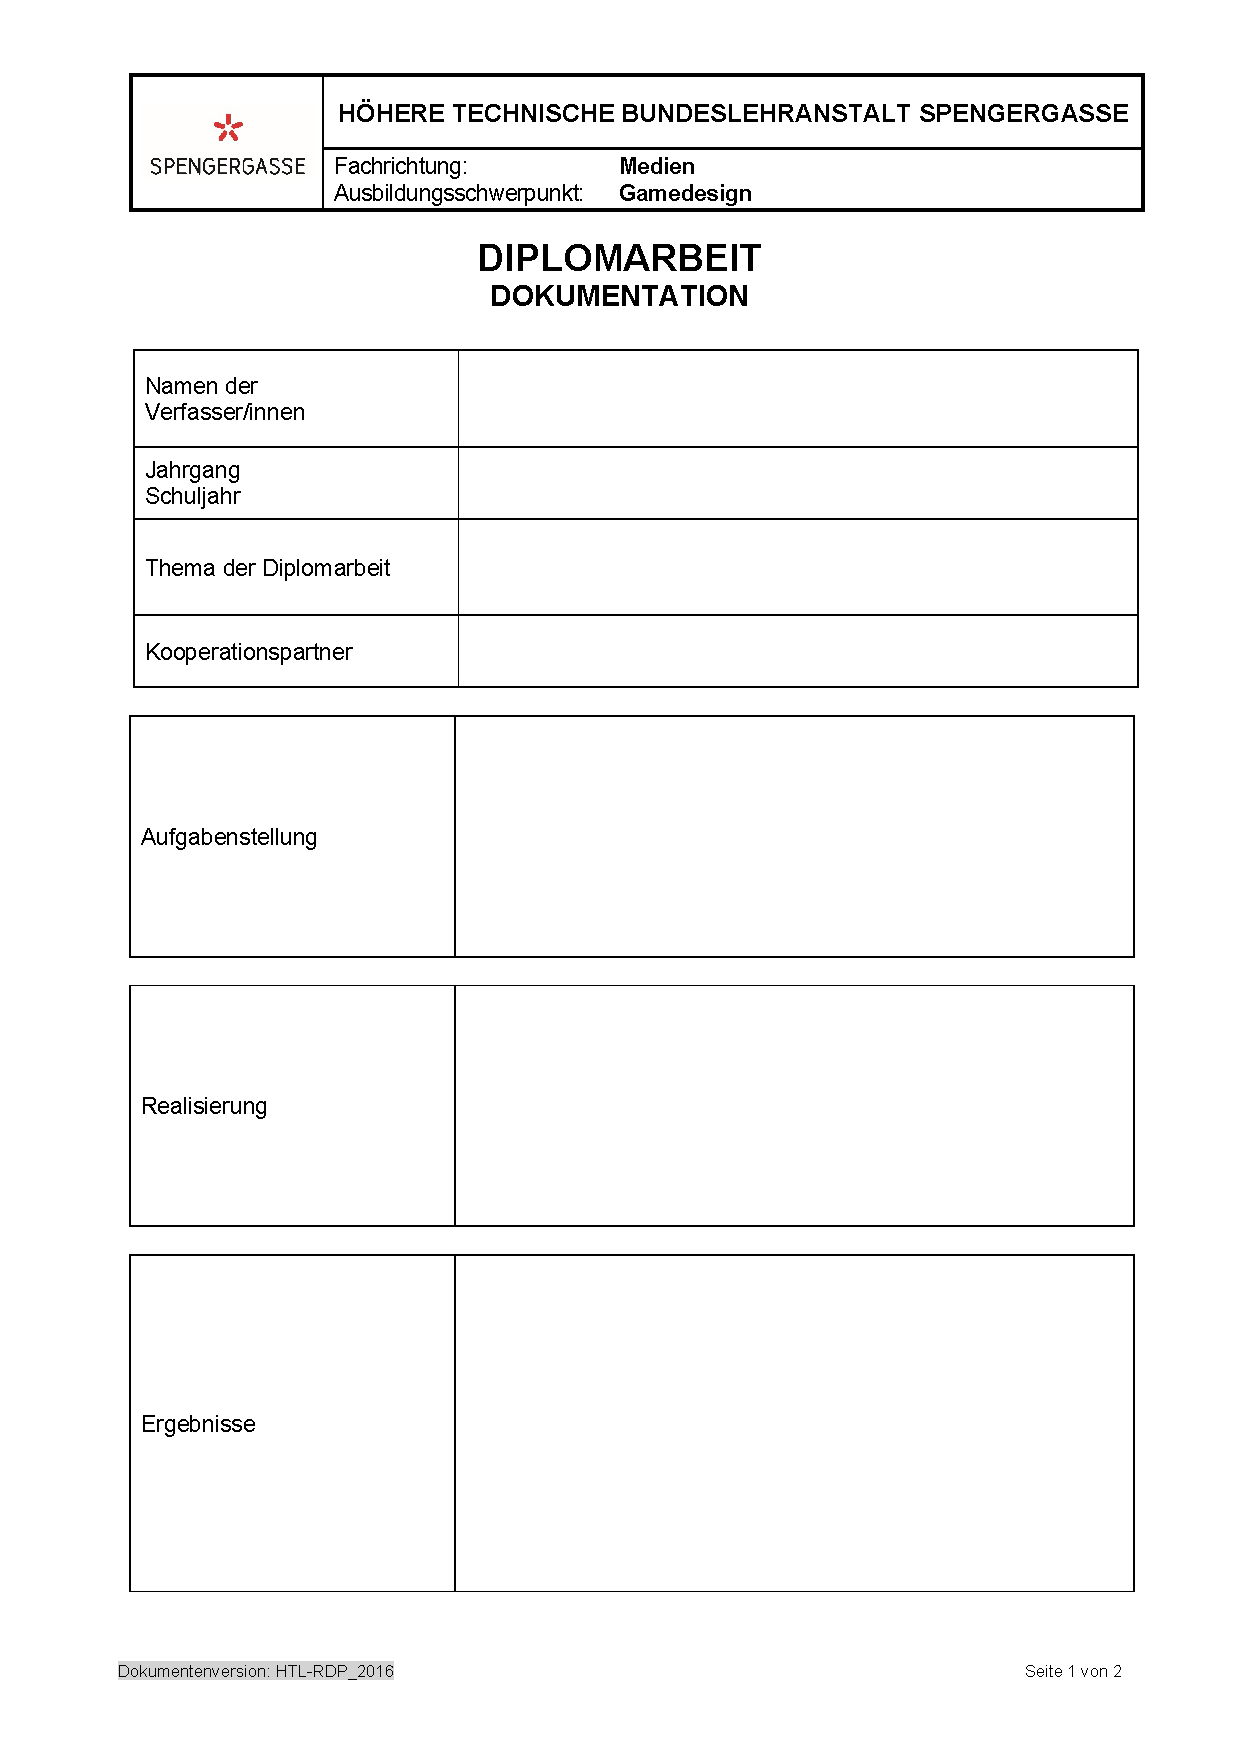
\includepdf[page=-]{formulare/HTL_RDP_Dokumentation_DA_DE_A4}
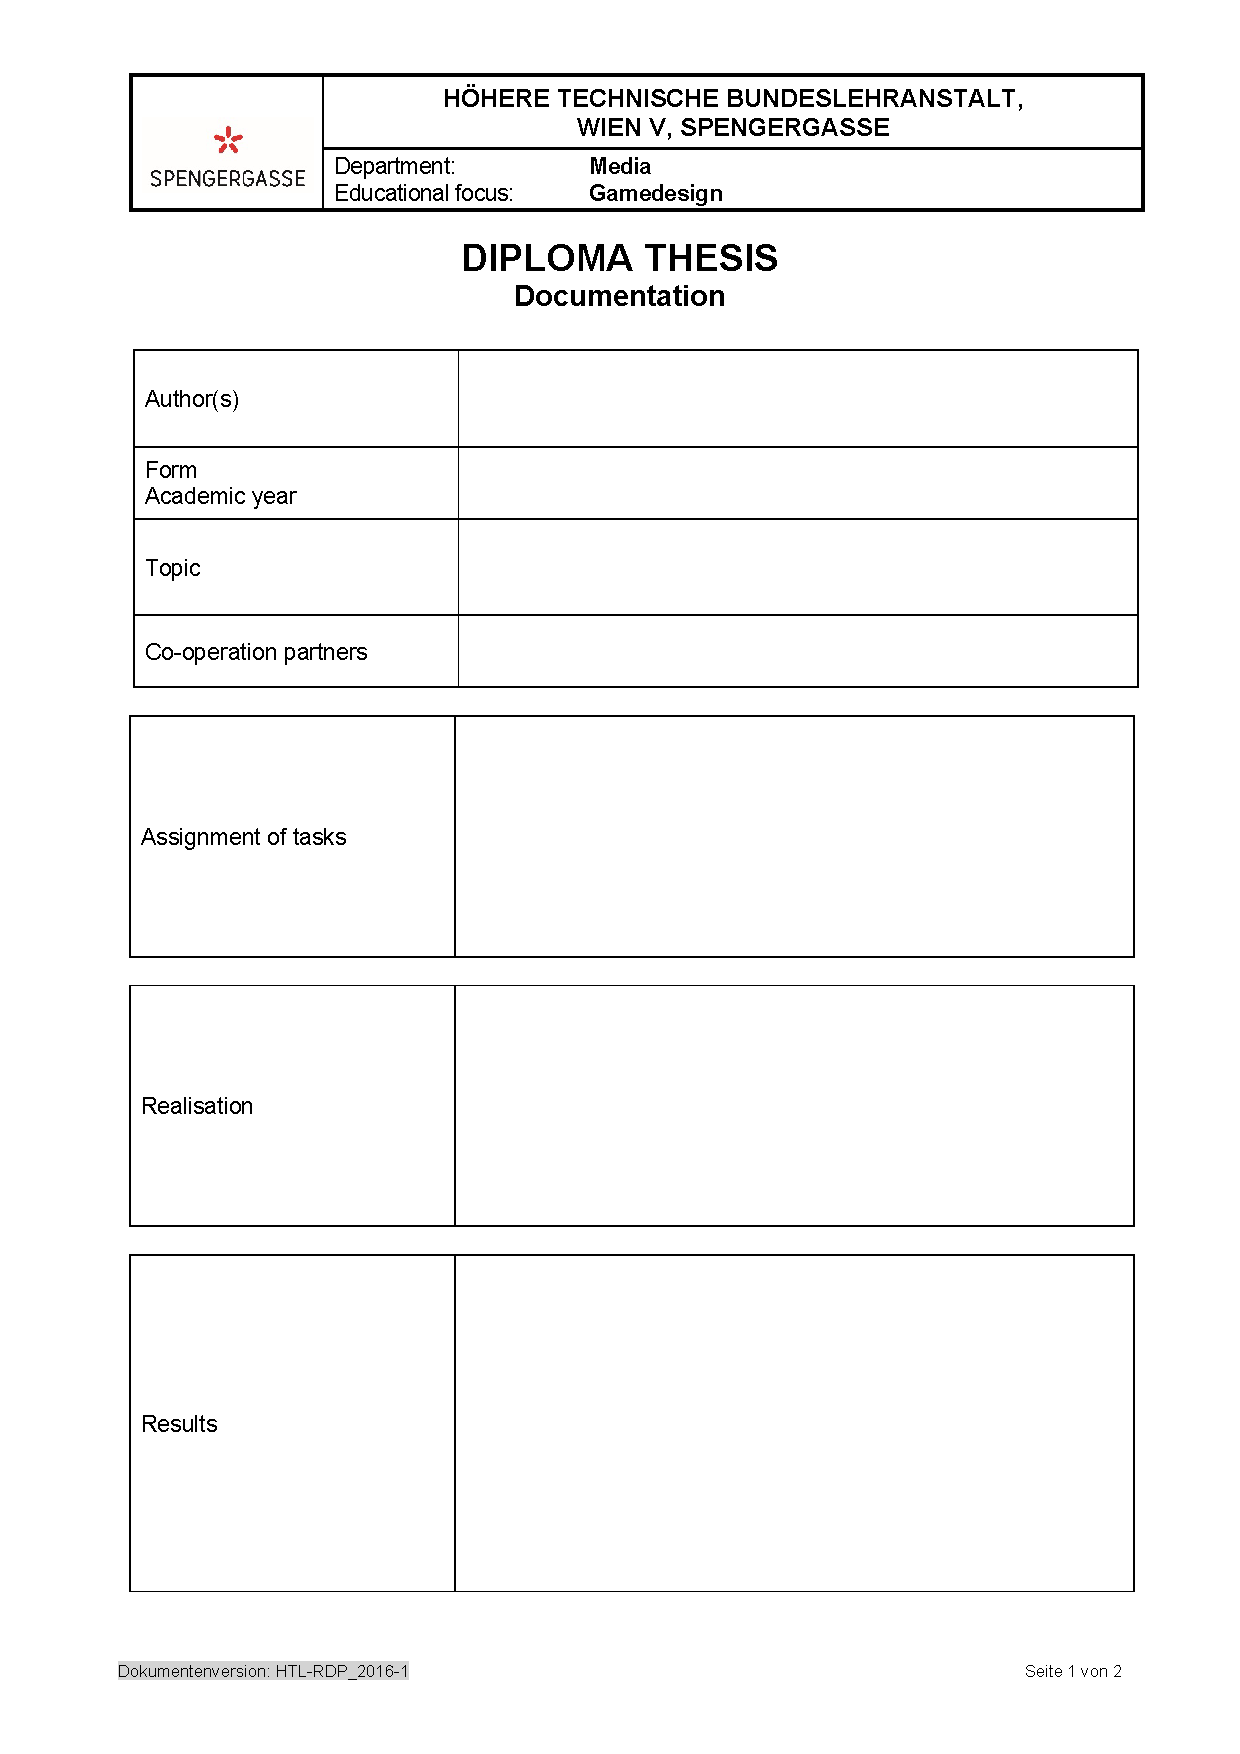
\includepdf[page=-]{formulare/HTL_RDP_Dokumentation_DA_EN_A4}
\cleardoublepage

\includepdf[page=-]{formulare/HTL_AP_Diplomarbeit_Eigenständigkeitserklärung}

%%%----------------------------------------------------------
\tableofcontents
\thispagestyle{plain} % fix page style for last page of TOC
%%%----------------------------------------------------------

\cleardoublepage
\chapter*{Kurzfassung}
\addcontentsline{toc}{chapter}{Kurzfassung}

An dieser Stelle steht eine Zusammenfassung der Arbeit, Umfang
max.\ 1 Seite. Im Unterschied zu anderen Kapiteln ist die
Kurzfassung (und das Abstract) üblicherweise nicht in Abschnitte
und Unterabschnitte gegliedert. 
Auch Fußnoten sind hier falsch am Platz.

Kurzfassungen werden übrigens häufig -- zusammen mit Autor und Titel
der Arbeit -- %
in Literaturdatenbanken aufgenommen. Es ist daher darauf zu
achten, dass die Information in der Kurzfassung für sich 
\emph{allein} (d.h. ohne weitere Teile der Arbeit) zusammenhängend und
abgeschlossen ist. Insbesondere werden an dieser Stelle (wie u.a.
auch im \emph{Titel} der Arbeit und im \emph{Abstract})
normalerweise \emph{keine Literaturverweise} verwendet! Falls man
unbedingt solche benötigt -- etwa weil die Arbeit eine
Weiterentwicklung einer bestimmten, früheren Arbeit darstellt --,
dann sind \emph{vollständige} Quellenangaben in der Kurzfassung
selbst notwendig, z.B. %
[\textsc{Zobel} J.: \textit{Writing for Computer Science -- The Art of
Effective Commu\-nica\-tion}. Springer-Verlag, Singa\-pur, 1997].

Weiters sollte man daran denken, dass bei der Aufnahme in Datenbanken
Sonderzeichen oder etwa Aufzählungen mit "Knödellisten" in der
Regel verloren gehen. Dasselbe gilt natürlich auch für das 
\emph{Abstract}.


Inhaltlich sollte die Kurzfassung \emph{keine} Auflistung der
einzelnen Kapitel sein (dafür ist das Einleitungskapitel
vorgesehen), sondern dem Leser einen kompakten, inhaltlichen
Überblick über die gesamte Arbeit verschaffen. Der hier verwendete
Aufbau ist daher zwangsläufig anders als der in der Einleitung.
   % vom Team gemeinsam zu verfassen
\cleardoublepage
\chapter*{Abstract}
\addcontentsline{toc}{chapter}{Abstract}

\begin{english} %switch to English language rules
This should be a 1-page (maximum) summary of your work in English.
\end{english}
%und hier geht dann das Abstract weiter...

Im englischen Abstract sollte inhaltlich das Gleiche
stehen wie in der deutschen Kurzfassung. Versuchen Sie daher, die
Kurzfassung prä\-zise umzusetzen, ohne aber dabei Wort für Wort zu
übersetzen. Beachten Sie bei der Übersetzung, dass gewisse
Redewendungen aus dem Deutschen im Englischen kein Pendant haben
oder völlig anders formuliert werden müssen und dass die
Satzstellung im Englischen sich (bekanntlich) vom Deutschen stark
unterscheidet. Es
empfiehlt sich übrigens -- auch bei höchstem Vertrauen in die
persönlichen Englischkenntnisse -- eine kundige Person für das
"proof reading" zu engagieren.

Die richtige Übersetzung für "Diplomarbeit" ist übrigens
schlicht \emph{thesis}, allenfalls  "diploma thesis" oder "Master's thesis", 
auf keinen Fall aber "diploma work" oder gar "dissertation".

		% vom Team gemeinsam in englisch zu verfassen	


%%%----------------------------------------------------------
% Hauptteil (ab hier arab. Seitenzahlen)
\cleardoublepage
\pagenumbering{arabic}
\pagestyle{fancy}
%%%----------------------------------------------------------  

% Trennseite erzeugt ein Titelblatt für eine neue Arbeit (zB wenn die Arbeit A endet und die Arbeit B beginnt)
% Parameter: {}Titel der Arbeit}{Autor}{Betreuer}{Abteilung}
% Beispiele: 
%	\trennseite{Gestaltpsychologie und stilisiertes Game Audio}{Noah Diem}{Dipl.Ing. Michael Schreiber}{Mediendesign - Gamedesign}
%	\trennseite{Collection and analysis of gameplay metrics}{Ian Hornik}{Mag. Andreas Metz}{Media design - Game design}

\trennseite{Grafische Optimierungsprozesse bei der Entwicklung eines minimalistischen Retro-Videospielstils}{SchuelerIn A}{Titel + Name Betreuer von Arbeit A}{Mediendesign - Gamedesign}
\chapter{Einleitung}
\label{cha:sa_Einleitung}

\section{Zielsetzung}
Dieses Dokument ist als vorwiegend technische Starthilfe für das
Erstellen einer Diplomarbeit mit \LaTeX
gedacht.

Das vorliegende Dokument dient einem zweifachen Zweck: 
\emph{erstens} als Erläuterung und Anleitung, \emph{zweitens} als
direkter Ausgangspunkt für die eigene Arbeit.


\section{Warum {\LaTeX}?}

Diplomarbeiten, Dissertationen und Bücher im
technisch-natur\-wissen\-schaft\-lichen Bereich werden
traditionell mithilfe des Textverarbeitungssystems \LaTeX
\cite{Lamport94,Lamport95} gesetzt.

Für den professionellen elektronischen Buchsatz wurde früher
häufig \emph{Adobe Framemaker} verwendet, allerdings ist diese
Software teuer und komplex. Eine modernere Alternative dazu ist
\emph{Adobe InDesign}, wobei allerdings die Erstellung
mathematischer Elemente und die Verwaltung von Literaturverweisen
zur Zeit nur rudimentär unterstützt werden.%
\footnote{Angeblich werden aber für den (sehr sauberen) Schriftsatz 
	in \emph{InDesign} ähnliche Algorithmen wie in \LaTeX\ verwendet.}

Microsoft \emph{Word} gilt im Unterschied zu \LaTeX, 
\emph{Framemaker} und \emph{InDesign} übrigens nicht als professionelle
Textverarbeitungssoftware, obwohl es immer häufiger auch von
großen Verlagen verwendet wird.%
\footnote{Siehe auch \url{http://latex.tugraz.at/mythen.php}.}
Das Schriftbild in \emph{Word}
lässt -- zumindest für das geschulte Auge -- einiges zu wünschen
übrig und das Erstellen von Büchern und ähnlich großen Dokumenten
wird nur unzureichend unterstützt. Allerdings ist \emph{Word} sehr
verbreitet, flexibel und vielen Benutzern zumindest oberflächlich
vertraut, sodass das Erlernen eines speziellen Werkzeugs wie
\LaTeX\ mühsam sein kann.

Übrigens, genau hier am Ende des Einleitungskapitels (und nicht
etwa in der Kurzfassung) ist der richtige Platz, um die
inhaltliche Gliederung der nachfolgenden Arbeit zu beschreiben.
Hier soll dargestellt werden, welche Teile (Kapitel) der Arbeit
welche Funktion haben und wie sie inhaltlich zusammenhängen. Auch
die Inhalte des \emph{Anhangs} -- sofern vorgesehen -- sollten hier
kurz beschrieben werden.


\chapter{Die Abschlussarbeit}
\label{cha:Diplomschrift}

Jede Diplomarbeit ist anders und dennoch sind sich gute
Arbeiten in ihrer Struktur meist sehr ähnlich, vor allem\ bei
technisch-natur\-wissen\-schaft\-lichen Themen. 

\section{Elemente der Abschlussarbeit}

Als Startpunkt bewährt hat sich die folgender
einfacher Grundaufbau, den man natürlich vari\-ieren und beliebig
verfeinern kann:
%
\begin{enumerate}
\item \textbf{Einführung und Motivation}: Was ist die Problem- oder Aufgabenstellung und
warum sollte man sich dafür interessieren?
\item \textbf{Präzisierung des Themas}: Hier beschreibt man den aktuellen Stand der Technik
oder Wissenschaft ("State-Of-The-Art"), zeigt bestehende
Defizite oder offene Fragen auf und entwickelt daraus die
Stoßrichtung der eigenen Arbeit.
\item \textbf{Eigener Ansatz}: Das ist natürlich der Kern der Arbeit. Hier
wird gezeigt, wie man die vorher beschriebene Aufgabenstellung löst und --
häufig in Form eines Programms%
\footnote{\emph{Prototyp} ist in diesem Zusammenhang ein gerne benutzter Begriff, der im Deutschen
allerdings oft unrichtig dekliniert wird. Richtig ist: der \emph{Prototyp}, des \emph{Prototyps}, dem/den \emph{Protototyp} -- falsch hingegen z.B.: des \emph{Prototyp\underline{en}}!
} --
realisiert, ergänzt durch illustrative Beispiele.
\item \textbf{Zusammenfassung}: Was wurde erreicht und welche Ziele sind
noch offen geblieben, wo könnte man weiter arbeiten?
\end{enumerate}
%
Natürlich ist auch ein gewisser dramaturgischer Aufbau der Arbeit
wichtig, wobei man bedenken muss, dass der Leser in der Regel nur
wenig Zeit hat und -- anders als etwa bei einem Roman -- seine
Geduld nicht auf die lange Folter gespannt werden darf. Erklären
Sie bereits in der Einführung (und nicht erst im letzten Kapitel),
wie Sie an die Sache herangehen, welche Lösungen Sie vorschlagen
und wie erfolgreich Sie damit waren.

Übrigens, auch Fehler und Sackgassen darf (und sollte) man
beschreiben; ihre Kenntnis hilft oft doppelte Experimente und
weitere Fehler zu vermeiden und ist damit sicher nützlicher als
jede Schönfärberei.
Und natürlich ist es auch nicht verboten, seine eigene Meinung 
in sachlicher Form zu äußern.


\section{Arbeiten in Englisch}
\label{sec:englisch}

Diese Vorlage ist zunächst darauf abgestellt, dass die
Diplomschrift in deutscher Sprache erstellt wird. Vor allem bei
Diplomarbeiten, die in Zusammenarbeit mit größeren Firmen oder
internationalen Instituten entstehen, ist es häufig erwünscht,
dass die Diplomschrift zu besseren Nutzbarkeit in englischer
Sprache verfasst wird, und viele Hochschulen%
\footnote{Die HTL Spengergasse macht hier keine Ausnahme.
} 
lassen dies in der Regel auch zu.

Beachten sollte man allerdings, dass das Schreiben dadurch nicht
einfacher wird, auch wenn einem Worte und Sätze im Englischen
scheinbar leichter "aus der Feder" fließen. Gerade im Bereich
der Informatik erscheint durch die Dominanz englischer
Fachausdrücke das Schreiben im Deutschen mühsam und das Ausweichen
ins Englische daher besonders attraktiv. Das ist jedoch
trügerisch, da man die eigene Fertigkeit in der Fremdsprache
(trotz der meist langjährigen Schulbildung) häufig überschätzt.
Prägnanz und Klarheit gehen leicht verloren und bisweilen ist das
Resultat ein peinliches Gefasel ohne Zusammenhang und soliden
Inhalt. Sofern man das Englische nicht wirklich gut beherrscht, ist
es ratsam, zumindest die wichtigsten Teile der Arbeit zunächst in
Deutsch zu verfassen und erst nachträglich zu übersetzen.
Besonders vorsichtig sollte man bei der Übersetzung von scheinbar
vertrauten Fachausdrücken sein. Zusätzlich ist es immer zu
empfehlen, die fertige Arbeit von einem "native speaker"
korrigieren zu lassen.


Technisch ist, außer der Spracheinstellung und den unterschiedlichen Anfüh\-rungszeichen, für eine englische Arbeit nicht viel zu ändern, allerdings sollte man folgendes beachten:
%
\begin{itemize}
\item  Die Titelseite (mit der Bezeichnung "Diplomarbeit") 
ist für die einzureichenden Exemplare jedenfalls in \emph{deutsch} zu halten,
auch wenn der Titel englisch ist. 
\item Ebenso muss neben dem
englischen \emph{Abstract} auch eine deutsche \emph{Kurzfassung}
enthalten sein. %
\item Akademische Titel von Personen haben im Englischen offenbar
weniger Bedeutung als im Deutschen und werden daher meist
weggelassen.
\end{itemize}


\trennseite{Measuring the Effect of Environmental Guidance Cues on Player Navigation in a Linear Game}{SchuelerIn B}{Titel + Name Betreuer von Arbeit A}{Mediendesign - Gamedesign}
\chapter{Einleitung}
\label{cha:sa_Einleitung}

\section{Zielsetzung}
Dieses Dokument ist als vorwiegend technische Starthilfe für das
Erstellen einer Diplomarbeit mit \LaTeX
gedacht.

Das vorliegende Dokument dient einem zweifachen Zweck: 
\emph{erstens} als Erläuterung und Anleitung, \emph{zweitens} als
direkter Ausgangspunkt für die eigene Arbeit.


\section{Warum {\LaTeX}?}

Diplomarbeiten, Dissertationen und Bücher im
technisch-natur\-wissen\-schaft\-lichen Bereich werden
traditionell mithilfe des Textverarbeitungssystems \LaTeX
\cite{Lamport94,Lamport95} gesetzt.

Für den professionellen elektronischen Buchsatz wurde früher
häufig \emph{Adobe Framemaker} verwendet, allerdings ist diese
Software teuer und komplex. Eine modernere Alternative dazu ist
\emph{Adobe InDesign}, wobei allerdings die Erstellung
mathematischer Elemente und die Verwaltung von Literaturverweisen
zur Zeit nur rudimentär unterstützt werden.%
\footnote{Angeblich werden aber für den (sehr sauberen) Schriftsatz 
	in \emph{InDesign} ähnliche Algorithmen wie in \LaTeX\ verwendet.}

Microsoft \emph{Word} gilt im Unterschied zu \LaTeX, 
\emph{Framemaker} und \emph{InDesign} übrigens nicht als professionelle
Textverarbeitungssoftware, obwohl es immer häufiger auch von
großen Verlagen verwendet wird.%
\footnote{Siehe auch \url{http://latex.tugraz.at/mythen.php}.}
Das Schriftbild in \emph{Word}
lässt -- zumindest für das geschulte Auge -- einiges zu wünschen
übrig und das Erstellen von Büchern und ähnlich großen Dokumenten
wird nur unzureichend unterstützt. Allerdings ist \emph{Word} sehr
verbreitet, flexibel und vielen Benutzern zumindest oberflächlich
vertraut, sodass das Erlernen eines speziellen Werkzeugs wie
\LaTeX\ mühsam sein kann.

Übrigens, genau hier am Ende des Einleitungskapitels (und nicht
etwa in der Kurzfassung) ist der richtige Platz, um die
inhaltliche Gliederung der nachfolgenden Arbeit zu beschreiben.
Hier soll dargestellt werden, welche Teile (Kapitel) der Arbeit
welche Funktion haben und wie sie inhaltlich zusammenhängen. Auch
die Inhalte des \emph{Anhangs} -- sofern vorgesehen -- sollten hier
kurz beschrieben werden.


\chapter{Die Abschlussarbeit}
\label{cha:Diplomschrift}

Jede Diplomarbeit ist anders und dennoch sind sich gute
Arbeiten in ihrer Struktur meist sehr ähnlich, vor allem\ bei
technisch-natur\-wissen\-schaft\-lichen Themen. 

\section{Elemente der Abschlussarbeit}

Als Startpunkt bewährt hat sich die folgender
einfacher Grundaufbau, den man natürlich vari\-ieren und beliebig
verfeinern kann:
%
\begin{enumerate}
\item \textbf{Einführung und Motivation}: Was ist die Problem- oder Aufgabenstellung und
warum sollte man sich dafür interessieren?
\item \textbf{Präzisierung des Themas}: Hier beschreibt man den aktuellen Stand der Technik
oder Wissenschaft ("State-Of-The-Art"), zeigt bestehende
Defizite oder offene Fragen auf und entwickelt daraus die
Stoßrichtung der eigenen Arbeit.
\item \textbf{Eigener Ansatz}: Das ist natürlich der Kern der Arbeit. Hier
wird gezeigt, wie man die vorher beschriebene Aufgabenstellung löst und --
häufig in Form eines Programms%
\footnote{\emph{Prototyp} ist in diesem Zusammenhang ein gerne benutzter Begriff, der im Deutschen
allerdings oft unrichtig dekliniert wird. Richtig ist: der \emph{Prototyp}, des \emph{Prototyps}, dem/den \emph{Protototyp} -- falsch hingegen z.B.: des \emph{Prototyp\underline{en}}!
} --
realisiert, ergänzt durch illustrative Beispiele.
\item \textbf{Zusammenfassung}: Was wurde erreicht und welche Ziele sind
noch offen geblieben, wo könnte man weiter arbeiten?
\end{enumerate}
%
Natürlich ist auch ein gewisser dramaturgischer Aufbau der Arbeit
wichtig, wobei man bedenken muss, dass der Leser in der Regel nur
wenig Zeit hat und -- anders als etwa bei einem Roman -- seine
Geduld nicht auf die lange Folter gespannt werden darf. Erklären
Sie bereits in der Einführung (und nicht erst im letzten Kapitel),
wie Sie an die Sache herangehen, welche Lösungen Sie vorschlagen
und wie erfolgreich Sie damit waren.

Übrigens, auch Fehler und Sackgassen darf (und sollte) man
beschreiben; ihre Kenntnis hilft oft doppelte Experimente und
weitere Fehler zu vermeiden und ist damit sicher nützlicher als
jede Schönfärberei.
Und natürlich ist es auch nicht verboten, seine eigene Meinung 
in sachlicher Form zu äußern.


\section{Arbeiten in Englisch}
\label{sec:englisch}

Diese Vorlage ist zunächst darauf abgestellt, dass die
Diplomschrift in deutscher Sprache erstellt wird. Vor allem bei
Diplomarbeiten, die in Zusammenarbeit mit größeren Firmen oder
internationalen Instituten entstehen, ist es häufig erwünscht,
dass die Diplomschrift zu besseren Nutzbarkeit in englischer
Sprache verfasst wird, und viele Hochschulen%
\footnote{Die HTL Spengergasse macht hier keine Ausnahme.
} 
lassen dies in der Regel auch zu.

Beachten sollte man allerdings, dass das Schreiben dadurch nicht
einfacher wird, auch wenn einem Worte und Sätze im Englischen
scheinbar leichter "aus der Feder" fließen. Gerade im Bereich
der Informatik erscheint durch die Dominanz englischer
Fachausdrücke das Schreiben im Deutschen mühsam und das Ausweichen
ins Englische daher besonders attraktiv. Das ist jedoch
trügerisch, da man die eigene Fertigkeit in der Fremdsprache
(trotz der meist langjährigen Schulbildung) häufig überschätzt.
Prägnanz und Klarheit gehen leicht verloren und bisweilen ist das
Resultat ein peinliches Gefasel ohne Zusammenhang und soliden
Inhalt. Sofern man das Englische nicht wirklich gut beherrscht, ist
es ratsam, zumindest die wichtigsten Teile der Arbeit zunächst in
Deutsch zu verfassen und erst nachträglich zu übersetzen.
Besonders vorsichtig sollte man bei der Übersetzung von scheinbar
vertrauten Fachausdrücken sein. Zusätzlich ist es immer zu
empfehlen, die fertige Arbeit von einem "native speaker"
korrigieren zu lassen.


Technisch ist, außer der Spracheinstellung und den unterschiedlichen Anfüh\-rungszeichen, für eine englische Arbeit nicht viel zu ändern, allerdings sollte man folgendes beachten:
%
\begin{itemize}
\item  Die Titelseite (mit der Bezeichnung "Diplomarbeit") 
ist für die einzureichenden Exemplare jedenfalls in \emph{deutsch} zu halten,
auch wenn der Titel englisch ist. 
\item Ebenso muss neben dem
englischen \emph{Abstract} auch eine deutsche \emph{Kurzfassung}
enthalten sein. %
\item Akademische Titel von Personen haben im Englischen offenbar
weniger Bedeutung als im Deutschen und werden daher meist
weggelassen.
\end{itemize}


\trennseite{Spatial Audio in atmospheric games}{SchuelerIn C}{Titel + Name Betreuer von Arbeit A}{Mediendesign - Gamedesign}
\chapter{Einleitung}
\label{cha:sa_Einleitung}

\section{Zielsetzung}
Dieses Dokument ist als vorwiegend technische Starthilfe für das
Erstellen einer Diplomarbeit mit \LaTeX
gedacht.

Das vorliegende Dokument dient einem zweifachen Zweck: 
\emph{erstens} als Erläuterung und Anleitung, \emph{zweitens} als
direkter Ausgangspunkt für die eigene Arbeit.


\section{Warum {\LaTeX}?}

Diplomarbeiten, Dissertationen und Bücher im
technisch-natur\-wissen\-schaft\-lichen Bereich werden
traditionell mithilfe des Textverarbeitungssystems \LaTeX
\cite{Lamport94,Lamport95} gesetzt.

Für den professionellen elektronischen Buchsatz wurde früher
häufig \emph{Adobe Framemaker} verwendet, allerdings ist diese
Software teuer und komplex. Eine modernere Alternative dazu ist
\emph{Adobe InDesign}, wobei allerdings die Erstellung
mathematischer Elemente und die Verwaltung von Literaturverweisen
zur Zeit nur rudimentär unterstützt werden.%
\footnote{Angeblich werden aber für den (sehr sauberen) Schriftsatz 
	in \emph{InDesign} ähnliche Algorithmen wie in \LaTeX\ verwendet.}

Microsoft \emph{Word} gilt im Unterschied zu \LaTeX, 
\emph{Framemaker} und \emph{InDesign} übrigens nicht als professionelle
Textverarbeitungssoftware, obwohl es immer häufiger auch von
großen Verlagen verwendet wird.%
\footnote{Siehe auch \url{http://latex.tugraz.at/mythen.php}.}
Das Schriftbild in \emph{Word}
lässt -- zumindest für das geschulte Auge -- einiges zu wünschen
übrig und das Erstellen von Büchern und ähnlich großen Dokumenten
wird nur unzureichend unterstützt. Allerdings ist \emph{Word} sehr
verbreitet, flexibel und vielen Benutzern zumindest oberflächlich
vertraut, sodass das Erlernen eines speziellen Werkzeugs wie
\LaTeX\ mühsam sein kann.

Übrigens, genau hier am Ende des Einleitungskapitels (und nicht
etwa in der Kurzfassung) ist der richtige Platz, um die
inhaltliche Gliederung der nachfolgenden Arbeit zu beschreiben.
Hier soll dargestellt werden, welche Teile (Kapitel) der Arbeit
welche Funktion haben und wie sie inhaltlich zusammenhängen. Auch
die Inhalte des \emph{Anhangs} -- sofern vorgesehen -- sollten hier
kurz beschrieben werden.


\chapter{Die Abschlussarbeit}
\label{cha:Diplomschrift}

Jede Diplomarbeit ist anders und dennoch sind sich gute
Arbeiten in ihrer Struktur meist sehr ähnlich, vor allem\ bei
technisch-natur\-wissen\-schaft\-lichen Themen. 

\section{Elemente der Abschlussarbeit}

Als Startpunkt bewährt hat sich die folgender
einfacher Grundaufbau, den man natürlich vari\-ieren und beliebig
verfeinern kann:
%
\begin{enumerate}
\item \textbf{Einführung und Motivation}: Was ist die Problem- oder Aufgabenstellung und
warum sollte man sich dafür interessieren?
\item \textbf{Präzisierung des Themas}: Hier beschreibt man den aktuellen Stand der Technik
oder Wissenschaft ("State-Of-The-Art"), zeigt bestehende
Defizite oder offene Fragen auf und entwickelt daraus die
Stoßrichtung der eigenen Arbeit.
\item \textbf{Eigener Ansatz}: Das ist natürlich der Kern der Arbeit. Hier
wird gezeigt, wie man die vorher beschriebene Aufgabenstellung löst und --
häufig in Form eines Programms%
\footnote{\emph{Prototyp} ist in diesem Zusammenhang ein gerne benutzter Begriff, der im Deutschen
allerdings oft unrichtig dekliniert wird. Richtig ist: der \emph{Prototyp}, des \emph{Prototyps}, dem/den \emph{Protototyp} -- falsch hingegen z.B.: des \emph{Prototyp\underline{en}}!
} --
realisiert, ergänzt durch illustrative Beispiele.
\item \textbf{Zusammenfassung}: Was wurde erreicht und welche Ziele sind
noch offen geblieben, wo könnte man weiter arbeiten?
\end{enumerate}
%
Natürlich ist auch ein gewisser dramaturgischer Aufbau der Arbeit
wichtig, wobei man bedenken muss, dass der Leser in der Regel nur
wenig Zeit hat und -- anders als etwa bei einem Roman -- seine
Geduld nicht auf die lange Folter gespannt werden darf. Erklären
Sie bereits in der Einführung (und nicht erst im letzten Kapitel),
wie Sie an die Sache herangehen, welche Lösungen Sie vorschlagen
und wie erfolgreich Sie damit waren.

Übrigens, auch Fehler und Sackgassen darf (und sollte) man
beschreiben; ihre Kenntnis hilft oft doppelte Experimente und
weitere Fehler zu vermeiden und ist damit sicher nützlicher als
jede Schönfärberei.
Und natürlich ist es auch nicht verboten, seine eigene Meinung 
in sachlicher Form zu äußern.


\section{Arbeiten in Englisch}
\label{sec:englisch}

Diese Vorlage ist zunächst darauf abgestellt, dass die
Diplomschrift in deutscher Sprache erstellt wird. Vor allem bei
Diplomarbeiten, die in Zusammenarbeit mit größeren Firmen oder
internationalen Instituten entstehen, ist es häufig erwünscht,
dass die Diplomschrift zu besseren Nutzbarkeit in englischer
Sprache verfasst wird, und viele Hochschulen%
\footnote{Die HTL Spengergasse macht hier keine Ausnahme.
} 
lassen dies in der Regel auch zu.

Beachten sollte man allerdings, dass das Schreiben dadurch nicht
einfacher wird, auch wenn einem Worte und Sätze im Englischen
scheinbar leichter "aus der Feder" fließen. Gerade im Bereich
der Informatik erscheint durch die Dominanz englischer
Fachausdrücke das Schreiben im Deutschen mühsam und das Ausweichen
ins Englische daher besonders attraktiv. Das ist jedoch
trügerisch, da man die eigene Fertigkeit in der Fremdsprache
(trotz der meist langjährigen Schulbildung) häufig überschätzt.
Prägnanz und Klarheit gehen leicht verloren und bisweilen ist das
Resultat ein peinliches Gefasel ohne Zusammenhang und soliden
Inhalt. Sofern man das Englische nicht wirklich gut beherrscht, ist
es ratsam, zumindest die wichtigsten Teile der Arbeit zunächst in
Deutsch zu verfassen und erst nachträglich zu übersetzen.
Besonders vorsichtig sollte man bei der Übersetzung von scheinbar
vertrauten Fachausdrücken sein. Zusätzlich ist es immer zu
empfehlen, die fertige Arbeit von einem "native speaker"
korrigieren zu lassen.


Technisch ist, außer der Spracheinstellung und den unterschiedlichen Anfüh\-rungszeichen, für eine englische Arbeit nicht viel zu ändern, allerdings sollte man folgendes beachten:
%
\begin{itemize}
\item  Die Titelseite (mit der Bezeichnung "Diplomarbeit") 
ist für die einzureichenden Exemplare jedenfalls in \emph{deutsch} zu halten,
auch wenn der Titel englisch ist. 
\item Ebenso muss neben dem
englischen \emph{Abstract} auch eine deutsche \emph{Kurzfassung}
enthalten sein. %
\item Akademische Titel von Personen haben im Englischen offenbar
weniger Bedeutung als im Deutschen und werden daher meist
weggelassen.
\end{itemize}


\trennseite{Entwicklung eines immersiven Charactercontrollers für isometrische Videospiele }{SchuelerIn C}{Titel + Name Betreuer von Arbeit A}{Mediendesign - Gamedesign}
\chapter{Einleitung}
\label{cha:sa_Einleitung}

\section{Zielsetzung}
Dieses Dokument ist als vorwiegend technische Starthilfe für das
Erstellen einer Diplomarbeit mit \LaTeX
gedacht.

Das vorliegende Dokument dient einem zweifachen Zweck: 
\emph{erstens} als Erläuterung und Anleitung, \emph{zweitens} als
direkter Ausgangspunkt für die eigene Arbeit.


\section{Warum {\LaTeX}?}

Diplomarbeiten, Dissertationen und Bücher im
technisch-natur\-wissen\-schaft\-lichen Bereich werden
traditionell mithilfe des Textverarbeitungssystems \LaTeX
\cite{Lamport94,Lamport95} gesetzt.

Für den professionellen elektronischen Buchsatz wurde früher
häufig \emph{Adobe Framemaker} verwendet, allerdings ist diese
Software teuer und komplex. Eine modernere Alternative dazu ist
\emph{Adobe InDesign}, wobei allerdings die Erstellung
mathematischer Elemente und die Verwaltung von Literaturverweisen
zur Zeit nur rudimentär unterstützt werden.%
\footnote{Angeblich werden aber für den (sehr sauberen) Schriftsatz 
	in \emph{InDesign} ähnliche Algorithmen wie in \LaTeX\ verwendet.}

Microsoft \emph{Word} gilt im Unterschied zu \LaTeX, 
\emph{Framemaker} und \emph{InDesign} übrigens nicht als professionelle
Textverarbeitungssoftware, obwohl es immer häufiger auch von
großen Verlagen verwendet wird.%
\footnote{Siehe auch \url{http://latex.tugraz.at/mythen.php}.}
Das Schriftbild in \emph{Word}
lässt -- zumindest für das geschulte Auge -- einiges zu wünschen
übrig und das Erstellen von Büchern und ähnlich großen Dokumenten
wird nur unzureichend unterstützt. Allerdings ist \emph{Word} sehr
verbreitet, flexibel und vielen Benutzern zumindest oberflächlich
vertraut, sodass das Erlernen eines speziellen Werkzeugs wie
\LaTeX\ mühsam sein kann.

Übrigens, genau hier am Ende des Einleitungskapitels (und nicht
etwa in der Kurzfassung) ist der richtige Platz, um die
inhaltliche Gliederung der nachfolgenden Arbeit zu beschreiben.
Hier soll dargestellt werden, welche Teile (Kapitel) der Arbeit
welche Funktion haben und wie sie inhaltlich zusammenhängen. Auch
die Inhalte des \emph{Anhangs} -- sofern vorgesehen -- sollten hier
kurz beschrieben werden.


\chapter{Die Abschlussarbeit}
\label{cha:Diplomschrift}

Jede Diplomarbeit ist anders und dennoch sind sich gute
Arbeiten in ihrer Struktur meist sehr ähnlich, vor allem\ bei
technisch-natur\-wissen\-schaft\-lichen Themen. 

\section{Elemente der Abschlussarbeit}

Als Startpunkt bewährt hat sich die folgender
einfacher Grundaufbau, den man natürlich vari\-ieren und beliebig
verfeinern kann:
%
\begin{enumerate}
\item \textbf{Einführung und Motivation}: Was ist die Problem- oder Aufgabenstellung und
warum sollte man sich dafür interessieren?
\item \textbf{Präzisierung des Themas}: Hier beschreibt man den aktuellen Stand der Technik
oder Wissenschaft ("State-Of-The-Art"), zeigt bestehende
Defizite oder offene Fragen auf und entwickelt daraus die
Stoßrichtung der eigenen Arbeit.
\item \textbf{Eigener Ansatz}: Das ist natürlich der Kern der Arbeit. Hier
wird gezeigt, wie man die vorher beschriebene Aufgabenstellung löst und --
häufig in Form eines Programms%
\footnote{\emph{Prototyp} ist in diesem Zusammenhang ein gerne benutzter Begriff, der im Deutschen
allerdings oft unrichtig dekliniert wird. Richtig ist: der \emph{Prototyp}, des \emph{Prototyps}, dem/den \emph{Protototyp} -- falsch hingegen z.B.: des \emph{Prototyp\underline{en}}!
} --
realisiert, ergänzt durch illustrative Beispiele.
\item \textbf{Zusammenfassung}: Was wurde erreicht und welche Ziele sind
noch offen geblieben, wo könnte man weiter arbeiten?
\end{enumerate}
%
Natürlich ist auch ein gewisser dramaturgischer Aufbau der Arbeit
wichtig, wobei man bedenken muss, dass der Leser in der Regel nur
wenig Zeit hat und -- anders als etwa bei einem Roman -- seine
Geduld nicht auf die lange Folter gespannt werden darf. Erklären
Sie bereits in der Einführung (und nicht erst im letzten Kapitel),
wie Sie an die Sache herangehen, welche Lösungen Sie vorschlagen
und wie erfolgreich Sie damit waren.

Übrigens, auch Fehler und Sackgassen darf (und sollte) man
beschreiben; ihre Kenntnis hilft oft doppelte Experimente und
weitere Fehler zu vermeiden und ist damit sicher nützlicher als
jede Schönfärberei.
Und natürlich ist es auch nicht verboten, seine eigene Meinung 
in sachlicher Form zu äußern.


\section{Arbeiten in Englisch}
\label{sec:englisch}

Diese Vorlage ist zunächst darauf abgestellt, dass die
Diplomschrift in deutscher Sprache erstellt wird. Vor allem bei
Diplomarbeiten, die in Zusammenarbeit mit größeren Firmen oder
internationalen Instituten entstehen, ist es häufig erwünscht,
dass die Diplomschrift zu besseren Nutzbarkeit in englischer
Sprache verfasst wird, und viele Hochschulen%
\footnote{Die HTL Spengergasse macht hier keine Ausnahme.
} 
lassen dies in der Regel auch zu.

Beachten sollte man allerdings, dass das Schreiben dadurch nicht
einfacher wird, auch wenn einem Worte und Sätze im Englischen
scheinbar leichter "aus der Feder" fließen. Gerade im Bereich
der Informatik erscheint durch die Dominanz englischer
Fachausdrücke das Schreiben im Deutschen mühsam und das Ausweichen
ins Englische daher besonders attraktiv. Das ist jedoch
trügerisch, da man die eigene Fertigkeit in der Fremdsprache
(trotz der meist langjährigen Schulbildung) häufig überschätzt.
Prägnanz und Klarheit gehen leicht verloren und bisweilen ist das
Resultat ein peinliches Gefasel ohne Zusammenhang und soliden
Inhalt. Sofern man das Englische nicht wirklich gut beherrscht, ist
es ratsam, zumindest die wichtigsten Teile der Arbeit zunächst in
Deutsch zu verfassen und erst nachträglich zu übersetzen.
Besonders vorsichtig sollte man bei der Übersetzung von scheinbar
vertrauten Fachausdrücken sein. Zusätzlich ist es immer zu
empfehlen, die fertige Arbeit von einem "native speaker"
korrigieren zu lassen.


Technisch ist, außer der Spracheinstellung und den unterschiedlichen Anfüh\-rungszeichen, für eine englische Arbeit nicht viel zu ändern, allerdings sollte man folgendes beachten:
%
\begin{itemize}
\item  Die Titelseite (mit der Bezeichnung "Diplomarbeit") 
ist für die einzureichenden Exemplare jedenfalls in \emph{deutsch} zu halten,
auch wenn der Titel englisch ist. 
\item Ebenso muss neben dem
englischen \emph{Abstract} auch eine deutsche \emph{Kurzfassung}
enthalten sein. %
\item Akademische Titel von Personen haben im Englischen offenbar
weniger Bedeutung als im Deutschen und werden daher meist
weggelassen.
\end{itemize}

\chapter{Isometrische Videospiele}
\label{cha:Diplomschrift}

Jede Diplomarbeit ist anders und dennoch sind sich gute
Arbeiten in ihrer Struktur meist sehr ähnlich, vor allem\ bei
technisch-natur\-wissen\-schaft\-lichen Themen. 

\section{Definition von isometrischen Videospielen}

Als Startpunkt bewährt hat sich die folgender
einfacher Grundaufbau, den man natürlich vari\-ieren und beliebig
verfeinern kann:
%
\begin{enumerate}
\item \textbf{Einführung und Motivation}: Was ist die Problem- oder Aufgabenstellung und
warum sollte man sich dafür interessieren?
\item \textbf{Präzisierung des Themas}: Hier beschreibt man den aktuellen Stand der Technik
oder Wissenschaft ("State-Of-The-Art"), zeigt bestehende
Defizite oder offene Fragen auf und entwickelt daraus die
Stoßrichtung der eigenen Arbeit.
\item \textbf{Eigener Ansatz}: Das ist natürlich der Kern der Arbeit. Hier
wird gezeigt, wie man die vorher beschriebene Aufgabenstellung löst und --
häufig in Form eines Programms%
\footnote{\emph{Prototyp} ist in diesem Zusammenhang ein gerne benutzter Begriff, der im Deutschen
allerdings oft unrichtig dekliniert wird. Richtig ist: der \emph{Prototyp}, des \emph{Prototyps}, dem/den \emph{Protototyp} -- falsch hingegen z.B.: des \emph{Prototyp\underline{en}}!
} --
realisiert, ergänzt durch illustrative Beispiele.
\item \textbf{Zusammenfassung}: Was wurde erreicht und welche Ziele sind
noch offen geblieben, wo könnte man weiter arbeiten?
\end{enumerate}
%
Natürlich ist auch ein gewisser dramaturgischer Aufbau der Arbeit
wichtig, wobei man bedenken muss, dass der Leser in der Regel nur
wenig Zeit hat und -- anders als etwa bei einem Roman -- seine
Geduld nicht auf die lange Folter gespannt werden darf. Erklären
Sie bereits in der Einführung (und nicht erst im letzten Kapitel),
wie Sie an die Sache herangehen, welche Lösungen Sie vorschlagen
und wie erfolgreich Sie damit waren.

Übrigens, auch Fehler und Sackgassen darf (und sollte) man
beschreiben; ihre Kenntnis hilft oft doppelte Experimente und
weitere Fehler zu vermeiden und ist damit sicher nützlicher als
jede Schönfärberei.
Und natürlich ist es auch nicht verboten, seine eigene Meinung 
in sachlicher Form zu äußern.


\section{Immersionskonzepte vergleichbarer Videospiele}
\label{sec:englisch}

Diese Vorlage ist zunächst darauf abgestellt, dass die
Diplomschrift in deutscher Sprache erstellt wird. Vor allem bei
Diplomarbeiten, die in Zusammenarbeit mit größeren Firmen oder
internationalen Instituten entstehen, ist es häufig erwünscht,
dass die Diplomschrift zu besseren Nutzbarkeit in englischer
Sprache verfasst wird, und viele Hochschulen%
\footnote{Die HTL Spengergasse macht hier keine Ausnahme.
} 
lassen dies in der Regel auch zu.

Beachten sollte man allerdings, dass das Schreiben dadurch nicht
einfacher wird, auch wenn einem Worte und Sätze im Englischen
scheinbar leichter "aus der Feder" fließen. Gerade im Bereich
der Informatik erscheint durch die Dominanz englischer
Fachausdrücke das Schreiben im Deutschen mühsam und das Ausweichen
ins Englische daher besonders attraktiv. Das ist jedoch
trügerisch, da man die eigene Fertigkeit in der Fremdsprache
(trotz der meist langjährigen Schulbildung) häufig überschätzt.
Prägnanz und Klarheit gehen leicht verloren und bisweilen ist das
Resultat ein peinliches Gefasel ohne Zusammenhang und soliden
Inhalt. Sofern man das Englische nicht wirklich gut beherrscht, ist
es ratsam, zumindest die wichtigsten Teile der Arbeit zunächst in
Deutsch zu verfassen und erst nachträglich zu übersetzen.
Besonders vorsichtig sollte man bei der Übersetzung von scheinbar
vertrauten Fachausdrücken sein. Zusätzlich ist es immer zu
empfehlen, die fertige Arbeit von einem "native speaker"
korrigieren zu lassen.


Technisch ist, außer der Spracheinstellung und den unterschiedlichen Anfüh\-rungszeichen, für eine englische Arbeit nicht viel zu ändern, allerdings sollte man folgendes beachten:
%
\begin{itemize}
\item  Die Titelseite (mit der Bezeichnung "Diplomarbeit") 
ist für die einzureichenden Exemplare jedenfalls in \emph{deutsch} zu halten,
auch wenn der Titel englisch ist. 
\item Ebenso muss neben dem
englischen \emph{Abstract} auch eine deutsche \emph{Kurzfassung}
enthalten sein. %
\item Akademische Titel von Personen haben im Englischen offenbar
weniger Bedeutung als im Deutschen und werden daher meist
weggelassen.
\end{itemize}

\section{Einfluss auf Spielersteuerung}

\section{Vor- und Nachteile isometrischer Perspektive}

\chapter{Umsetzung einer immersiven isometrischen Spielersteuerung}
\label{cha:Diplomschrift}

Jede Diplomarbeit ist anders und dennoch sind sich gute
Arbeiten in ihrer Struktur meist sehr ähnlich, vor allem\ bei
technisch-natur\-wissen\-schaft\-lichen Themen. 

\section{Konzeption der Steuerung}

Als Startpunkt bewährt hat sich die folgender
einfacher Grundaufbau, den man natürlich vari\-ieren und beliebig
verfeinern kann:
%
\begin{enumerate}
\item \textbf{Einführung und Motivation}: Was ist die Problem- oder Aufgabenstellung und
warum sollte man sich dafür interessieren?
\item \textbf{Präzisierung des Themas}: Hier beschreibt man den aktuellen Stand der Technik
oder Wissenschaft ("State-Of-The-Art"), zeigt bestehende
Defizite oder offene Fragen auf und entwickelt daraus die
Stoßrichtung der eigenen Arbeit.
\item \textbf{Eigener Ansatz}: Das ist natürlich der Kern der Arbeit. Hier
wird gezeigt, wie man die vorher beschriebene Aufgabenstellung löst und --
häufig in Form eines Programms%
\footnote{\emph{Prototyp} ist in diesem Zusammenhang ein gerne benutzter Begriff, der im Deutschen
allerdings oft unrichtig dekliniert wird. Richtig ist: der \emph{Prototyp}, des \emph{Prototyps}, dem/den \emph{Protototyp} -- falsch hingegen z.B.: des \emph{Prototyp\underline{en}}!
} --
realisiert, ergänzt durch illustrative Beispiele.
\item \textbf{Zusammenfassung}: Was wurde erreicht und welche Ziele sind
noch offen geblieben, wo könnte man weiter arbeiten?
\end{enumerate}
%
Natürlich ist auch ein gewisser dramaturgischer Aufbau der Arbeit
wichtig, wobei man bedenken muss, dass der Leser in der Regel nur
wenig Zeit hat und -- anders als etwa bei einem Roman -- seine
Geduld nicht auf die lange Folter gespannt werden darf. Erklären
Sie bereits in der Einführung (und nicht erst im letzten Kapitel),
wie Sie an die Sache herangehen, welche Lösungen Sie vorschlagen
und wie erfolgreich Sie damit waren.

Übrigens, auch Fehler und Sackgassen darf (und sollte) man
beschreiben; ihre Kenntnis hilft oft doppelte Experimente und
weitere Fehler zu vermeiden und ist damit sicher nützlicher als
jede Schönfärberei.
Und natürlich ist es auch nicht verboten, seine eigene Meinung 
in sachlicher Form zu äußern.


\section{Bewegung des Spielers}
\label{sec:englisch}

Diese Vorlage ist zunächst darauf abgestellt, dass die
Diplomschrift in deutscher Sprache erstellt wird. Vor allem bei
Diplomarbeiten, die in Zusammenarbeit mit größeren Firmen oder
internationalen Instituten entstehen, ist es häufig erwünscht,
dass die Diplomschrift zu besseren Nutzbarkeit in englischer
Sprache verfasst wird, und viele Hochschulen%
\footnote{Die HTL Spengergasse macht hier keine Ausnahme.
} 
lassen dies in der Regel auch zu.

Beachten sollte man allerdings, dass das Schreiben dadurch nicht
einfacher wird, auch wenn einem Worte und Sätze im Englischen
scheinbar leichter "aus der Feder" fließen. Gerade im Bereich
der Informatik erscheint durch die Dominanz englischer
Fachausdrücke das Schreiben im Deutschen mühsam und das Ausweichen
ins Englische daher besonders attraktiv. Das ist jedoch
trügerisch, da man die eigene Fertigkeit in der Fremdsprache
(trotz der meist langjährigen Schulbildung) häufig überschätzt.
Prägnanz und Klarheit gehen leicht verloren und bisweilen ist das
Resultat ein peinliches Gefasel ohne Zusammenhang und soliden
Inhalt. Sofern man das Englische nicht wirklich gut beherrscht, ist
es ratsam, zumindest die wichtigsten Teile der Arbeit zunächst in
Deutsch zu verfassen und erst nachträglich zu übersetzen.
Besonders vorsichtig sollte man bei der Übersetzung von scheinbar
vertrauten Fachausdrücken sein. Zusätzlich ist es immer zu
empfehlen, die fertige Arbeit von einem "native speaker"
korrigieren zu lassen.


Technisch ist, außer der Spracheinstellung und den unterschiedlichen Anfüh\-rungszeichen, für eine englische Arbeit nicht viel zu ändern, allerdings sollte man folgendes beachten:
%
\begin{itemize}
\item  Die Titelseite (mit der Bezeichnung "Diplomarbeit") 
ist für die einzureichenden Exemplare jedenfalls in \emph{deutsch} zu halten,
auch wenn der Titel englisch ist. 
\item Ebenso muss neben dem
englischen \emph{Abstract} auch eine deutsche \emph{Kurzfassung}
enthalten sein. %
\item Akademische Titel von Personen haben im Englischen offenbar
weniger Bedeutung als im Deutschen und werden daher meist
weggelassen.
\end{itemize}

\section{Kamerasteuerung}

\section{Feedbacksysteme}

\chapter{Evaluation der Immersion}
\label{cha:Diplomschrift}

Jede Diplomarbeit ist anders und dennoch sind sich gute
Arbeiten in ihrer Struktur meist sehr ähnlich, vor allem\ bei
technisch-natur\-wissen\-schaft\-lichen Themen. 

\section{Entwicklung des Testkonzepts}

Als Startpunkt bewährt hat sich die folgender
einfacher Grundaufbau, den man natürlich vari\-ieren und beliebig
verfeinern kann:
%
\begin{enumerate}
\item \textbf{Einführung und Motivation}: Was ist die Problem- oder Aufgabenstellung und
warum sollte man sich dafür interessieren?
\item \textbf{Präzisierung des Themas}: Hier beschreibt man den aktuellen Stand der Technik
oder Wissenschaft ("State-Of-The-Art"), zeigt bestehende
Defizite oder offene Fragen auf und entwickelt daraus die
Stoßrichtung der eigenen Arbeit.
\item \textbf{Eigener Ansatz}: Das ist natürlich der Kern der Arbeit. Hier
wird gezeigt, wie man die vorher beschriebene Aufgabenstellung löst und --
häufig in Form eines Programms%
\footnote{\emph{Prototyp} ist in diesem Zusammenhang ein gerne benutzter Begriff, der im Deutschen
allerdings oft unrichtig dekliniert wird. Richtig ist: der \emph{Prototyp}, des \emph{Prototyps}, dem/den \emph{Protototyp} -- falsch hingegen z.B.: des \emph{Prototyp\underline{en}}!
} --
realisiert, ergänzt durch illustrative Beispiele.
\item \textbf{Zusammenfassung}: Was wurde erreicht und welche Ziele sind
noch offen geblieben, wo könnte man weiter arbeiten?
\end{enumerate}
%
Natürlich ist auch ein gewisser dramaturgischer Aufbau der Arbeit
wichtig, wobei man bedenken muss, dass der Leser in der Regel nur
wenig Zeit hat und -- anders als etwa bei einem Roman -- seine
Geduld nicht auf die lange Folter gespannt werden darf. Erklären
Sie bereits in der Einführung (und nicht erst im letzten Kapitel),
wie Sie an die Sache herangehen, welche Lösungen Sie vorschlagen
und wie erfolgreich Sie damit waren.

Übrigens, auch Fehler und Sackgassen darf (und sollte) man
beschreiben; ihre Kenntnis hilft oft doppelte Experimente und
weitere Fehler zu vermeiden und ist damit sicher nützlicher als
jede Schönfärberei.
Und natürlich ist es auch nicht verboten, seine eigene Meinung 
in sachlicher Form zu äußern.


\section{Durchführung der Spieltests}
\label{sec:englisch}

Diese Vorlage ist zunächst darauf abgestellt, dass die
Diplomschrift in deutscher Sprache erstellt wird. Vor allem bei
Diplomarbeiten, die in Zusammenarbeit mit größeren Firmen oder
internationalen Instituten entstehen, ist es häufig erwünscht,
dass die Diplomschrift zu besseren Nutzbarkeit in englischer
Sprache verfasst wird, und viele Hochschulen%
\footnote{Die HTL Spengergasse macht hier keine Ausnahme.
} 
lassen dies in der Regel auch zu.

Beachten sollte man allerdings, dass das Schreiben dadurch nicht
einfacher wird, auch wenn einem Worte und Sätze im Englischen
scheinbar leichter "aus der Feder" fließen. Gerade im Bereich
der Informatik erscheint durch die Dominanz englischer
Fachausdrücke das Schreiben im Deutschen mühsam und das Ausweichen
ins Englische daher besonders attraktiv. Das ist jedoch
trügerisch, da man die eigene Fertigkeit in der Fremdsprache
(trotz der meist langjährigen Schulbildung) häufig überschätzt.
Prägnanz und Klarheit gehen leicht verloren und bisweilen ist das
Resultat ein peinliches Gefasel ohne Zusammenhang und soliden
Inhalt. Sofern man das Englische nicht wirklich gut beherrscht, ist
es ratsam, zumindest die wichtigsten Teile der Arbeit zunächst in
Deutsch zu verfassen und erst nachträglich zu übersetzen.
Besonders vorsichtig sollte man bei der Übersetzung von scheinbar
vertrauten Fachausdrücken sein. Zusätzlich ist es immer zu
empfehlen, die fertige Arbeit von einem "native speaker"
korrigieren zu lassen.


Technisch ist, außer der Spracheinstellung und den unterschiedlichen Anfüh\-rungszeichen, für eine englische Arbeit nicht viel zu ändern, allerdings sollte man folgendes beachten:
%
\begin{itemize}
\item  Die Titelseite (mit der Bezeichnung "Diplomarbeit") 
ist für die einzureichenden Exemplare jedenfalls in \emph{deutsch} zu halten,
auch wenn der Titel englisch ist. 
\item Ebenso muss neben dem
englischen \emph{Abstract} auch eine deutsche \emph{Kurzfassung}
enthalten sein. %
\item Akademische Titel von Personen haben im Englischen offenbar
weniger Bedeutung als im Deutschen und werden daher meist
weggelassen.
\end{itemize}

\section{Bewertung der Immersion}

\section{Diskussion der Ergebnisse}
% falls es englische Arbeiten gibt, können englische Bereiche der Arbeit mit \begin{english} und \end{english} umschlossen werden.
%\begin{english}
%\trennseite{Collection and analysis of gameplay metrics}{Ian Hornik}{Mag. Andreas Metz}{Media design - Game design}
%\include{hornik/hornik}
%\end{english}

%\trennseite{Titel der Arbeit B}{SchuelerIn D}{Titel + Name Betreuer von Arbeit B}{Mediendesign - Gamedesign}
%\chapter{Einleitung}
\label{cha:sb_Einleitung}

\section{Zielsetzung}
Dieses Dokument ist als vorwiegend technische Starthilfe für das
Erstellen einer Diplomarbeit mit \LaTeX\ gedacht.

Das vorliegende Dokument dient einem zweifachen Zweck: 
\emph{erstens} als Erläuterung und Anleitung, \emph{zweitens} als
direkter Ausgangspunkt für die eigene Arbeit.


\section{Warum {\LaTeX}?}

Diplomarbeiten, Dissertationen und Bücher im
technisch-natur\-wissen\-schaft\-lichen Bereich werden
traditionell mithilfe des Textverarbeitungssystems \LaTeX\ 
\cite{Lamport94,Lamport95} gesetzt.

Für den professionellen elektronischen Buchsatz wurde früher
häufig \emph{Adobe Framemaker} verwendet, allerdings ist diese
Software teuer und komplex. Eine modernere Alternative dazu ist
\emph{Adobe InDesign}, wobei allerdings die Erstellung
mathematischer Elemente und die Verwaltung von Literaturverweisen
zur Zeit nur rudimentär unterstützt werden.%
\footnote{Angeblich werden aber für den (sehr sauberen) Schriftsatz 
in \emph{InDesign} ähnliche Algorithmen wie in \LaTeX\ verwendet.}

Microsoft \emph{Word} gilt im Unterschied zu \LaTeX, 
\emph{Framemaker} und \emph{InDesign} übrigens nicht als professionelle
Textverarbeitungssoftware, obwohl es immer häufiger auch von
großen Verlagen verwendet wird.%
\footnote{Siehe auch \url{http://latex.tugraz.at/mythen.php}.}
Das Schriftbild in \emph{Word}
lässt -- zumindest für das geschulte Auge -- einiges zu wünschen
übrig und das Erstellen von Büchern und ähnlich großen Dokumenten
wird nur unzureichend unterstützt. Allerdings ist \emph{Word} sehr
verbreitet, flexibel und vielen Benutzern zumindest oberflächlich
vertraut, sodass das Erlernen eines speziellen Werkzeugs wie
\LaTeX\ mühsam sein kann.

Übrigens, genau hier am Ende des Einleitungskapitels (und nicht
etwa in der Kurzfassung) ist der richtige Platz, um die
inhaltliche Gliederung der nachfolgenden Arbeit zu beschreiben.
Hier soll dargestellt werden, welche Teile (Kapitel) der Arbeit
welche Funktion haben und wie sie inhaltlich zusammenhängen. Auch
die Inhalte des \emph{Anhangs} -- sofern vorgesehen -- sollten hier
kurz beschrieben werden.


%\chapter{Abbildungen, Tabellen, Quellcode}
\label{chap:Abbildungen}

\section{Allgemeines}

Abbildungen (\emph{figures}) und Tabellen (\emph{tables}) werden üblicherweise
zusammen mit einem nummerierten Titel (\emph{caption}) zentriert
angeordnet (siehe Abb.~\ref{fig:CocaCola}).
Im Text \emph{muss} es zu jeder Abbildung einen Verweis geben und die eigentliche Abbildung
sollte erst \emph{nach} dem ersten Verweis platziert werden.

\begin{figure}
\centering
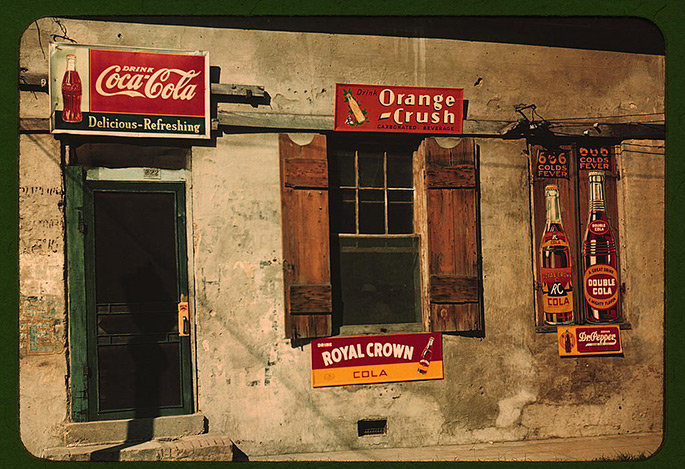
\includegraphics[width=.95\textwidth]{cola-public-domain-photo-p} %{CS0031}
\caption{Coca-Cola Werbung 1940 \cite{CocaCola1940}.}
\label{fig:CocaCola}
\end{figure}


\section{\emph{Let Them Float!}}

Das Platzieren von Abbildungen und Tabellen gehört zu den
schwierigsten Aufgaben im Schriftsatz, weil diese meist viel Platz
benötigen und häufig nicht auf der aktuellen Seite im laufenden
Text untergebracht werden können. Diese Elemente müssen daher an
eine geeignete Stelle auf nachfolgenden Seiten verschoben werden,
was manuell sehr mühsam (jedoch in \emph{Word} beispielsweise unerlässlich) ist.

In \LaTeX\ funktioniert das weitgehend automatisch, indem
Abbildungen, Tabellen und ähnliche als "Floating Bodies"
behandelt werden. Bei der Positionierung dieser Elemente wird
versucht, einerseits im Textfluss möglichst wenig Leer\-raum
entstehen zu lassen und andererseits die Abbildungen und Tabellen
nicht zu weit von der ursprünglichen Textstelle zu entfernen.

Der Gedanke, dass etwa Abbildungen kaum jemals genau an der
ge\-wünsch\-ten Stelle und möglicherweise nicht einmal auf
derselben Seite Platz finden, ist für viele Anfänger aber offenbar sehr
ungewohnt oder sogar beängstigend. Dennoch sollte man zunächst einmal
getrost \LaTeX\ diese Arbeit überlassen und \emph{nicht} manuell
eingreifen. Erst am Ende, wenn das gesamte Dokument "steht" und
man mit der automatischen Platzierung wirklich nicht zurande
kommt, sollte man (durch gezielte Platzierungsanweisungen
\cite[S.~33]{Oetiker01}) \textbf{in Einzelfällen} eingreifen.



\section{Captions}

Bei Abbildungen steht der Titel üblicherweise \emph{unten}, bei
Tabellen hingegen -- je nach Konvention -- \emph{oben} (wie in diesem Dokument) 
oder ebenfalls \emph{unten}. In \LaTeX\ erfolgt
auch die Nummerierung der Abbildungen automatisch, ebenso der
Eintrag in das (optionale)
Abbildungsverzeichnis%
\footnote{Ein eigenes Verzeichnis der Abbildungen am Anfang des Dokuments
ist zwar leicht erstellt, in einer Diplomarbeit aber (und eigentlich
überall sonst auch) überflüssig. Man sollte es daher weglassen.}
am Beginn des Dokuments.

Die Markierung der Captions%
\footnote{Ausnahmsweise wird das Wort "Caption" im Folgenden
ohne deutsche Übersetzung verwendet.} erfolgt in \LaTeX mithilfe
der \verb!\label{}! Anweisung, die unmittelbar auf die
\verb!\caption{}! Anweisung folgen muss:
%
\begin{lstlisting}[language={[LaTeX]TeX},basicstyle=\small,numbers=left]
\begin{figure}
\centering
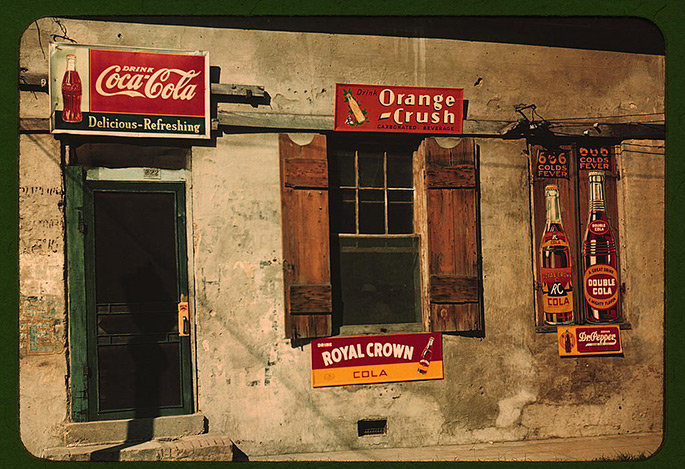
\includegraphics[width=.95\textwidth]{cola-public-domain-photo-p}
\caption{Coca-Cola Werbung 1940 \cite{CocaCola1940}.}
\label{fig:CocaCola}
\end{figure}
\end{lstlisting}
%
Der Name des Labels (\texttt{fig:CocaCola}) kann beliebig gewählt werden. 
Die Kennzeichnung \texttt{fig:} ist nur eine nützliche Hilfe, um beim Schreiben verschiedene Arten 
von Labels besser unterscheiden zu können.

Die Länge der Captions kann dabei sehr unterschiedlich sein. Je
nach Anwendung und Stil ergibt sich manchmal eine sehr kurze
Caption (Abb.~\ref{fig:CocaCola}) oder eine längere
(Abb.~\ref{fig:ibm360}).
Man beachte, wie bei kurzen Captions ein
zentrierter Satz und bei langen Captions ein Blocksatz verwendet
wird (\LaTeX\ macht das automatisch).
Captions sollten \emph{immer} mit einem Punkt abgeschlossen sein.%
\footnote{Kurioserweise verlangen manche Anleitungen
genau das Gegenteil, angeblich, weil beim klassischen Bleisatz 
die abschließenden Punkte im Druck häufig "weggebrochen" sind. 
Das kann man glauben oder nicht, im Digitaldruck 
spielt es jedenfalls keine Rolle.}

\begin{figure}
\centering
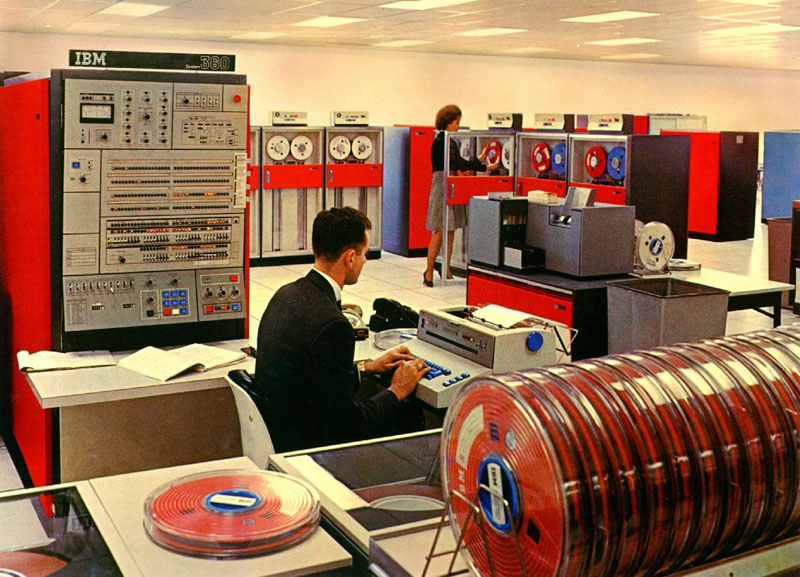
\includegraphics[width=.85\textwidth]{ibm-360-color}
\caption{Beispiel für einen langen Caption-Text. \textsc{Univac}
brachte 1961 mit dem Modell 751 den ersten Hochleistungsrechner
mit Halbleiterspeicher auf den Markt. Von diesem Computer wurden
in den U.S.A.\ bereits im ersten Produktionsjahr über fünfzig
Exemplare verkauft, vorwiegend an militärische Dienststellen,
Versicherungen und Großbanken. Die Ablöse erfolgte zwei Jahre
später durch das zusammen mit \textsc{Sperry} entwickelte Modell 820.
Das klingt vielleicht plausibel, ist aber völliger Unsinn, denn das
Bild zeigt in Wirklichkeit eine System/360 Anlage von IBM. 
Bildquelle~\cite{IBM360}.} 
\label{fig:ibm360}
\end{figure}




\section{Abbildungen}

Für die Einbindung von Grafiken in \LaTeX\ wird die Verwendung des Stan\-dard-Pakets
\texttt{graphicx} \cite{Carlisle99} empfohlen. 
Mit dem aktuell verwendeten Workflow (\texttt{pdflatex})
können Bild- bzw.\ Grafikformate ausschließlich 
in folgenden Formaten eingebunden werden:
%
\begin{itemize}
	\item \textbf{PNG}: für Grau-, S/W- und Farb-Rasterbilder (bevorzugt),
	\item \textbf{JPEG}: für Fotos (wenn nicht anders vorhanden),
	\item \textbf{PDF}: für Vektorgrafiken (Illustrationen, Strichzeichnungen etc.).
\end{itemize}
%
Bei Rasterbildern sollte wenn möglich PNG verwendet werden, weil die darin 
enthaltenen Bilder verlustfrei komprimiert sind und daher keine sichtbaren Kompressionsartefakte
aufweisen. Im Gegensatz dazu sollte man JPEG nur dann verwenden, wenn das Originalmaterial
(Foto) bereits in dieser Form vorliegt.


\subsection{Wo liegen die Grafikdateien?} 

Die Bilder werden üblicherweise in einem Unterverzeichnis (oder in mehreren Unterverzeichnissen) abgelegt,
im Fall dieses Dokuments in \nolinkurl{images/}.
Dazu dient die folgende Anweisung
am Beginn des Hauptdokuments \nolinkurl{_Diplomarbeit.tex}:
%
\begin{quote}
\verb!\graphicspath{{images/}}!
\end{quote}
%
Der (zum Hauptdokument relative) Pfad \texttt{graphicspath} kann innerhalb des
Dokuments jederzeit geändert werden, was durchaus nützlich ist, wenn man
z.B.\ die Grafiken einzelner Kapitel getrennt in entsprechenden Verzeichnissen
ablegen möchte.
Die Größe der Abbildung im Druck kann durch Vorgabe einer bestimmten
Breite oder Höhe oder eines Skalierungsfaktors gesteuert werden, z.B.:
%
\begin{quote}
\verb!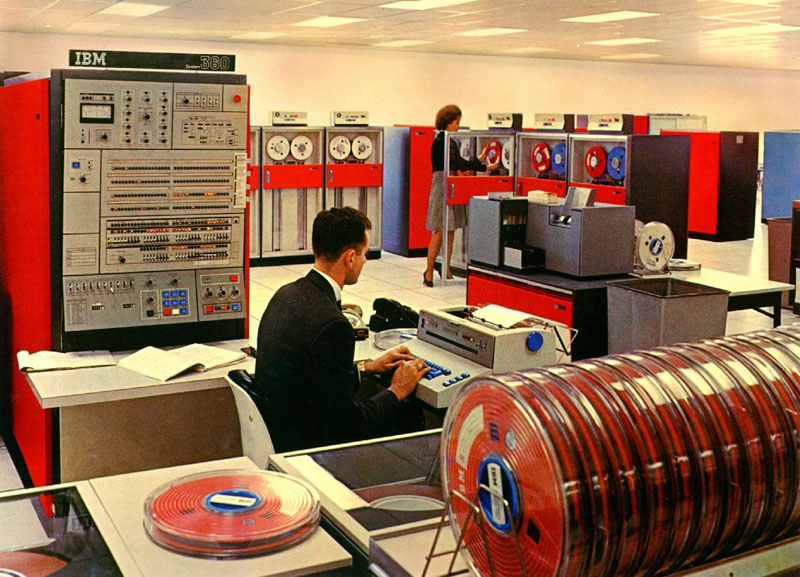
\includegraphics[width=.85\textwidth]{ibm-360-color}! \\
\verb!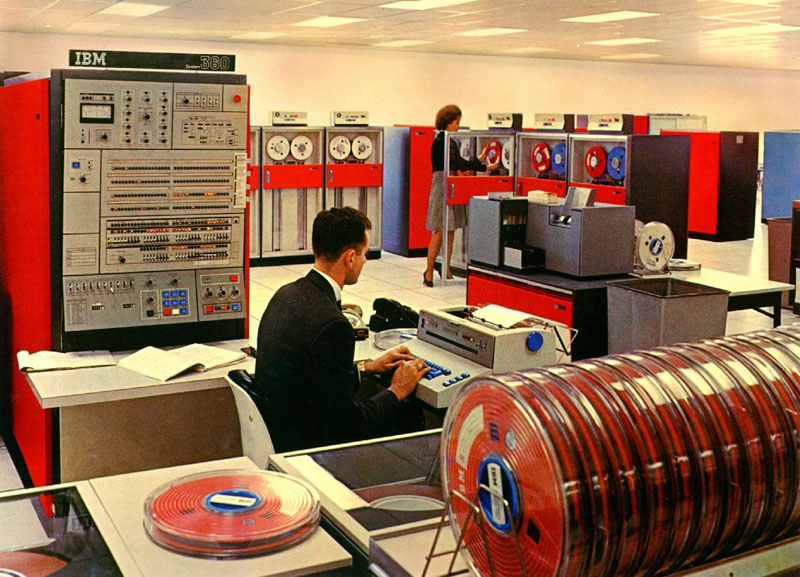
\includegraphics[scale=1.5]{ibm-360-color}!
\end{quote}
%
Man beachte, dass dabei die Dateiendung nicht explizit angegeben werden muss. 
Das ist vor allem dann praktisch, wenn man verschiedene Workflows mit jeweils
unterschiedlichen Dateitypen verwendet.


\subsection{Grafiken einrahmen} 

Mit dem Befehl \verb!\fbox{}! kann man optional einen dünnen 
Rahmen rund um die Grafik erzeugen, z.B.:
%
\begin{quote}
\verb!\fbox{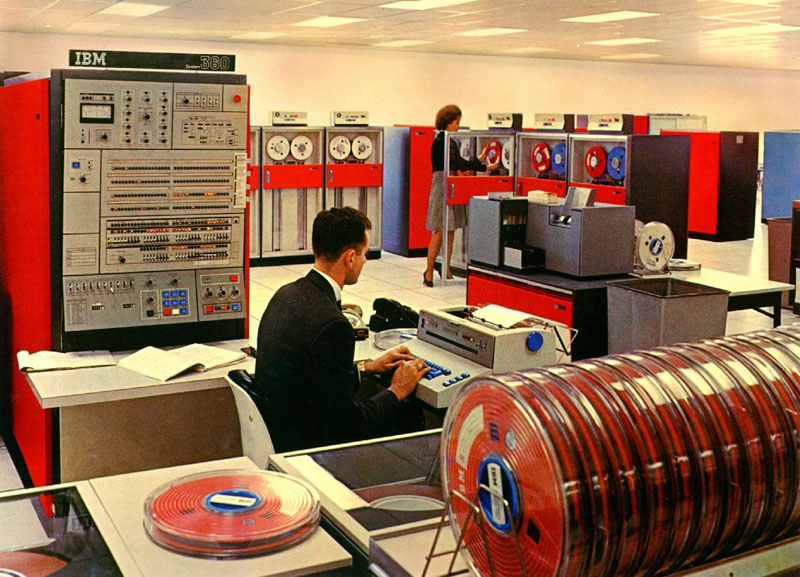
\includegraphics[height=50mm]{ibm-360-color}}!
\end{quote}
%
Das wird man üblicherweise nur bei Rasterbildern tun, insbesondere wenn sie zum Rand hin sehr hell sind
und ohne Rahmen nicht vom Hintergrund abgrenzbar wären.

\subsection{Rasterbilder (Pixelgrafiken)}

Generell sollte man Bilder bereits vorher so aufbereiten,
dass sie später beim Druck möglichst wenig an Qualität verlieren.
Es empfiehlt sich daher, die Bildgröße (Auflösung) bereits im Vorhinein
(z.B. mit \emph{Photoshop})
richtig einzustellen.
Brauchbare Auflösungen bezogen auf die endgültige Bildgröße sind:
%
\begin{itemize}
  \item \textbf{Farb- und Grauwertbilder:} 150--300 dpi
  \item \textbf{Binärbilder (Schwarz/Weiß):} 300--600 dpi
\end{itemize}
%
Eine wesentlich höhere Auflösung macht aufgrund der beim Laserdruck notwendigen
Rasterung keinen Sinn, auch bei 1200 dpi-Druckern.
Speziell \emph{Screen\-shots} sollte man nicht zu klein darstellen,
da sie sonst schlecht lesbar sind (max.\ 200 dpi, besser 150 dpi).
Dabei ist zu bedenken, dass die Arbeit auch als Kopie in allen
Details noch gut lesbar sein sollte.

\subsubsection{JPEG-Problematik}

In der Regel sollte man Bilder, die für den Einsatz in
Druckdokumenten gedacht sind, nicht mit verlustbehafteten
Kompressionsverfahren abspeichern. Insbesondere sollte man die Verwendung
von JPEG möglichst vermeiden, auch wenn viele Dateien dadurch
wesentlich kleiner werden. 
Eine Ausnahme ist, wenn die Originaldaten nur in JPEG vorliegen und für die 
Einbindung nicht bearbeitet oder verkleinert wurden. Ansonsten sollte man immer
PNG verwenden.

Besonders gerne werden farbige \textbf{Screenshots} einer JPEG-Kompression%
\footnote{Das JPEG-Verfahren ist für natürliche Fotos konzipiert und dafür auch gut geeignet,
seine undifferenzierte Verwendung ist aber zu einer globalen Plage geworden.}
unterzogen, obwohl deren verheerende Folgen auch für jeden Laien sichtbar sein sollten
(Abb.~\ref{fig:jpeg-pfusch}).

\begin{figure}
\centering\small
\begin{tabular}{cc}
\fbox{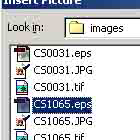
\includegraphics[width=0.45\textwidth]{screenshot-dirty}} &		% JPEG file
\fbox{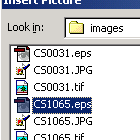
\includegraphics[width=0.45\textwidth]{screenshot-clean}} \\	% PNG file
(a) & (b) 
\end{tabular}
\caption{Typischer JPEG-Pfusch. Screenshots und ähnliche im Original
verfügbare Rasterbilder sollten für Druckdokumente \emph{keinesfalls} mit
JPEG komprimiert werden. Das Ergebnis~(a) sieht gegenüber dem
unkomprimierten Original~(b) nicht nur schmutzig aus, sondern wird
im Druck auch schnell unleserlich.} 
\label{fig:jpeg-pfusch}
\end{figure}






\subsection{Vektorgrafiken}

Für schematische Abbildungen (z.B. Flussdiagramme, Entity-Relationship-Diagramme
oder sonstige strukturelle Darstellungen) sollte man unbedingt
Vektorgrafiken (PDF) verwenden. % (\zB Abb.~\ref{fig:latex-pdf-workflow}).
Gerasterte Grafiken, wie man sie üblicherweise als GIF- oder PNG-Dateien
auf Webseiten findet, haben in einem Druckdokument nichts zu suchen, notfalls
muss man sie mit einem entsprechenden Werkzeug \emph{neu} zeichnen (natürlich
unter Angabe der ursprünglichen Quelle).

In diesem Fall kommt als Datenformat nur PDF %(oder EPS im DVI-PS-Workflow) 
in Frage,
dieses bietet sich aber auch in anderen Umgebungen als universelles
Vektor-Format an.
Zur Erstellung von PDF-Vektorgrafiken benötigt man ein geeignetes
Grafikprogramm, z.B. \emph{Freehand} %von \emph{Macromedia}
oder \emph{Illustrator} von \emph{Adobe}.
Manche gängige Grafikprogramme 
unterstützen allerdings keinen direkten Export von PDF-Dateien
oder erzeugen unsaubere Dateien. Vor der Entscheidung
für eine bestimmte Zeichensoftware sollte man das im Zweifelsfall
ausprobieren.
PDF kann im Notfall über einen entsprechenden Druckertreiber erzeugt werden.




\subsubsection{Einbettung von Schriften}

Die Wiedergabe von Textelementen ist abhängig von der auf dem
Computer (oder Drucker) installierten Schriften und der Form der
Schrifteinbettung im Quelldokument. Die korrekte Darstellung am
Bildschirm eines Computers bedeutet nicht, dass dasselbe Dokument
auf einem anderen Computer oder Drucker genau so dargestellt wird.
Dieser Umstand ist besonders wichtig, wenn Druckdokumente online
zur Verfügung gestellt werden. Kontrollieren Sie daher genau, ob
die innerhalb Ihrer Grafiken verwendeten Schriften auch exakt wie
beabsichtigt im Ausdruck aufscheinen.


%\chapter{Tabellen und Code}
Tabellen werden häufig eingesetzt um numerische Zusammenhänge, Testergebnisse
etc.\ in übersichtlicher Form darzustellen. Ein einfaches Beispiel ist Tab.~\ref{tab:processors}.

\begin{table}
	\caption{Prozessor-Familien im Überblick.}
	\label{tab:processors}
	\centering
	\setlength{\tabcolsep}{5mm}	% separator between columns
	\def\arraystretch{1.25}			% vertical stretch factor (Standard = 1.0)
	\begin{tabular}{|r||c|c|c|} \hline
		& \emph{PowerPC} & \emph{Pentium} & \emph{Athlon} \\
		\hline\hline
		Manufacturer & Motorola & Intel & AMD \\
		\hline
		Speed & high & medium & high   \\
		\hline
		Price & high & high   & medium \\
		\hline
	\end{tabular}
\end{table}



%%%----------------------------------------------------------
%%%Anhang
\appendix
\chapter{Projektdokumentation}

\section{Meilensteine}

\subsection{Meilenstein-Bezeichnung (TT. Monat JJJJ)}
To be done.

\subsection{Meilenstein-Bezeichnung (TT. Monat JJJJ)}
To be done.

\subsection{Meilenstein-Bezeichnung (TT. Monat JJJJ)}
To be done.

\subsection{Meilenstein-Bezeichnung (TT. Monat JJJJ)}
To be done.

\subsection{Goldmaster (TT. Monat JJJJ)}
To be done.

\section{Burndown}
\begin{figure}[ht]
	\centering
	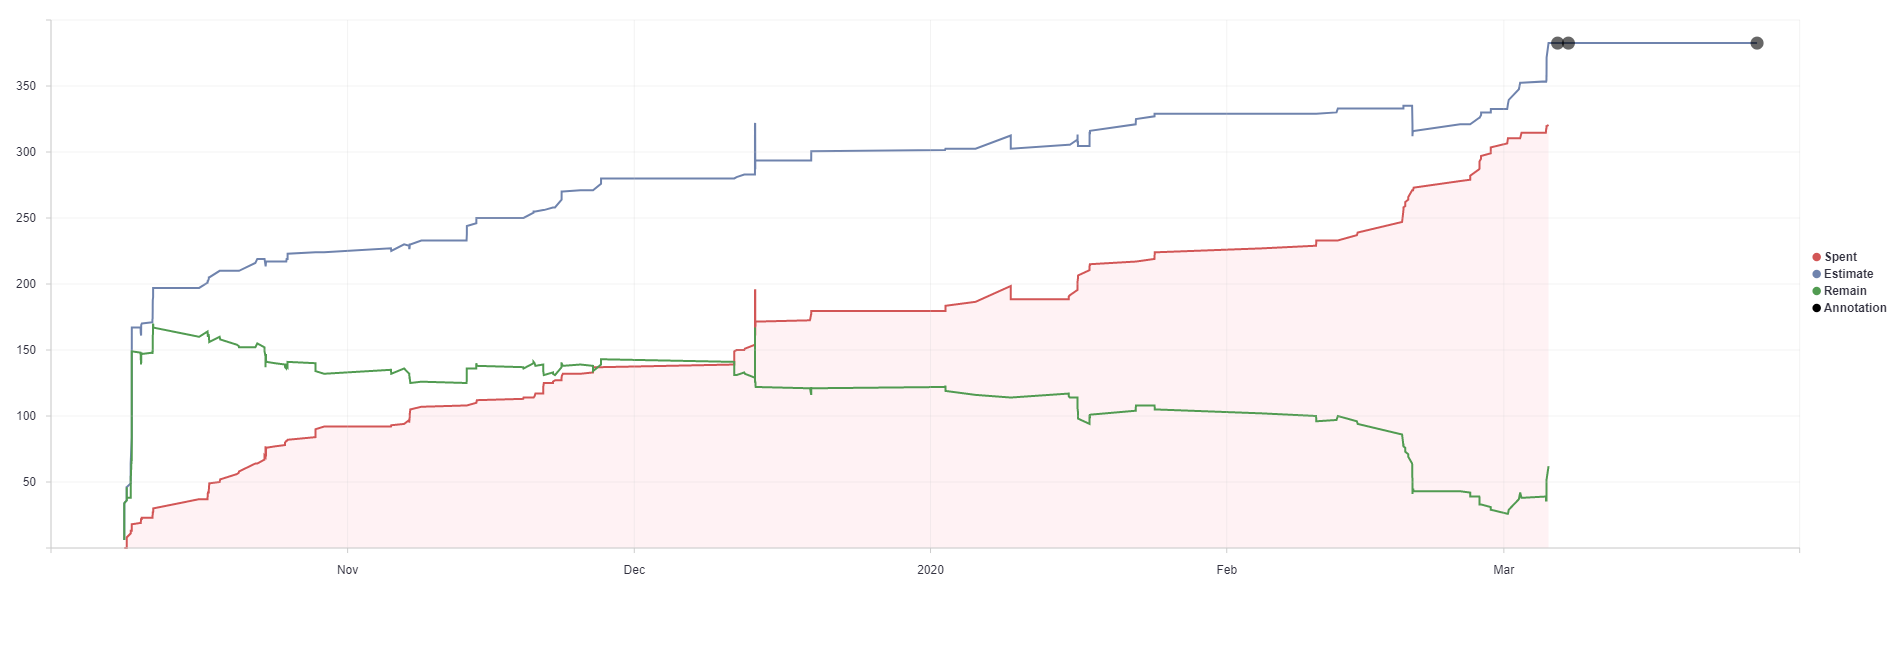
\includegraphics[width=0.9\textwidth]{burndown}
	\caption{Burndown chart}
\end{figure}

\section{Playtest Protokolle \& Ergebnisse}
To be done.
%\includepdf[page=-]{formulare/PlaytestProtokolle}

\section{Begleitprotokolle}
To be done.
%\includepdf[page=-]{formulare/Zeitprotokolle}	    % Projektdokumentation
\chapter{Kooperationsvereinbarung}

%\includepdf[page=-]{formulare/Kooperationsvereinbarung}	% Kooperationsvereinbarung
\chapter{Inhalt des Datenträgers}

\section{Projektdateien}

\section{PDF-Dateien} %zB gespeicherte Webseiten / Quellen
\begin{FileList}{/}
	\fitem{_Diplomarbeit.pdf} Diplomarbeit (Gesamtdokument)
	\fitem{Decisions.pdf} Artikel über Meaningful Decisions
\end{FileList}
 

\section{Presskit} % Ordner mit dem Presskit
	            % Inhalt des Datenträgers

%%%----------------------------------------------------------

\printbibliography
\addcontentsline{toc}{chapter}{Abbildungsverzeichnis}
\listoffigures
\addcontentsline{toc}{chapter}{Tabellenverzeichnis}
\listoftables

\end{document}
